\documentclass{article}

\usepackage[english]{babel}

% Set page size and margins
\usepackage[a4paper,top=2cm,bottom=2cm,left=3cm,right=3cm,marginparwidth=1.75cm]{geometry}

% Useful packages
\usepackage{amsmath}
\usepackage{graphicx}
\usepackage[colorlinks=true, allcolors=blue]{hyperref}
\usepackage{color}
\usepackage{minted}
\usepackage{tikz}
\usepackage{placeins}
\usepackage{float}
\usepackage[utf8]{inputenc}
\usepackage[T1]{fontenc}
\usepackage{fullpage}
\usepackage[numbers]{natbib}
\usepackage{minted}
\usepackage{amsmath,amssymb,amsfonts}
\usepackage{algorithmic}
\usepackage{graphicx}
\usepackage{textcomp}
\usepackage{placeins}
\usepackage{tabularx}
\usepackage{svg}

\setkeys{Gin}{width=\linewidth,totalheight=\textheight,keepaspectratio}

% Credit to Steven B. Segletes on StackExchange
% https://tex.stackexchange.com/a/265804

\usepackage[most]{tcolorbox}
\definecolor{block-gray}{gray}{0.85}
\newtcolorbox{myquote}{colback=block-gray,grow to right by=-10mm,grow to left by=-10mm, boxrule=0pt,boxsep=0pt,breakable}
\makeatletter
\def\quoteparse{\@ifnextchar`{\quotex}{\singlequote}}
\def\quotex#1{\@ifnextchar`{\triplequote\@gobble}{\doublequote}}
\makeatother
\def\singlequote#1`{\texttt{#1}\quoteON}
\def\doublequote#1``{\texttt{#1}\quoteON}
\long\def\triplequote#1```{\begin{myquote}\parskip 1ex#1\end{myquote}\quoteON}
\def\quoteON{\catcode``=\active}
\def\quoteOFF{\catcode``=12}
\quoteON
\def`{\quoteOFF \quoteparse}
\quoteOFF



\usepackage[outputDir=project/assingment1report,citations,hybrid]{markdown}

% Thanks to leandriis on StackOverflow for this formatting https://tex.stackexchange.com/a/533609
\usetikzlibrary{positioning,shapes.misc, shapes.geometric, arrows}


\tikzstyle{arrow} = [thick,->,>=stealth]
\tikzstyle{tCircle} = [circle, draw=black, align=center, minimum width=2cm]
\tikzstyle{tRoundRect} = [rounded rectangle, draw=black, align=center, minimum width=3cm, minimum height=1cm, text centered]
\tikzstyle{tRect} = [rectangle, draw=black, align=center, minimum width=3cm, minimum height=1cm, text centered]

\title{Your Title goes here}
\author{2100816}
\begin{document}
\maketitle
\quoteON

\begin{table}[h]
    \centering
    \begin{tabular}{ll}
        Registration number: & \textcolor{red}{2100816}\\
        Project: & \textcolor{red}{Causal inference}\\
        Link to GitHub: & \url{https://github.com/11BelowStudio/ce888}\\
    \end{tabular}
\end{table}



\begin{table}[h]
    \centering
    \begin{tabular}{lc}
        Executive summary (max.\ 250 words) & \textcolor{red}{Your word count}\\
        Introduction (max.\ 600 words) & \textcolor{red}{Your word count}\\
        Data (max.\ 500 words/dataset) & \textcolor{red}{Your word count}\\
        Methodology (max.\ 600 words) & \textcolor{red}{Your word count}\\
        Conclusions (max.\ 500 words) & \textcolor{red}{Your word count}\\
        \hline
        Total word count & \textcolor{red}{Your word count}\\
    \end{tabular}
    %\caption{Word counts for each section.}
\end{table}

\tableofcontents

\clearpage



\begin{abstract}
Your executive summary goes here.
\end{abstract}


\section{Introduction}

Your introduction goes here! Simply start writing your document and use the
Recompile button to view the updated PDF preview.

Examples of commonly used commands and features are listed below, in
Section~\ref{sec:tutorial}, to help you get started.
Instructions on what to include in each section are given in the assignment description

\href{https://moodle.essex.ac.uk/draftfile.php/196919/user/draft/666046553/2021_CE888_Assignment_1.pdf}{here}.

\section{Data}

This project involves two datasets: IHDP\cite{Gross1993} \cite{BROOKSGUNN1992350}  and JOBS\cite{JOBS_LaLonde}.

\subsection{IHDP - The Infant Health Development Program}

\FloatBarrier

* premature infants

* x: measurements taken when the kid was born, along with info about the home situation/what the mother was doing during pregnancy

* y: IQ test results

This dataset concerns a population of 750 individuals, all of whom have 25 \texttt{x} values,
a \texttt{t} value indicating whether they were in the treatment/control group, as well as
a factual \texttt{yf} value (indicating the true \texttt{y} value recorded from that individual
during the experiment), and a counterfactual \texttt{ycf} value (derived via a simulation,
simulating the outcome for that individual if they were in the opposite treatment/control group to
the group they actually were in). There is also an \texttt{ite} value, providing the individual
treatment effect for the individuals. The \texttt{y} values are continuous values.

Due to the presence of counterfactuals, one could consider this dataset to be balanced,
however, I shall not be using these in the training process for the investigation.
Therefore, I shall still need to treat this dataset as unbalanced,
with a total of 747 individuals; 608 in the control group, 139 in the treatment group.

A visualization of this dataset can be seen in \ref{fig:ihdpgraphs} (along with an overview
of the factual data within \ref{fig:ihdpfact}, and of the counterfactual data within \ref{fig:ihdpcf}).


Of the 25 'x' values, 6 of them are in a continuous range, whilst the other 19 are binary.
One of these non-binary 'x' values, \texttt{x3} , appears to be limited to one of four discrete
values; however, as I have been unable to conclusively find out what \texttt{x3} truly means,
and as that means it could possibly have a different value, I shall not normalize that into
discrete values, to allow leeway for potential future data, which may have a different value.


\begin{figure}[ht]
\centering
    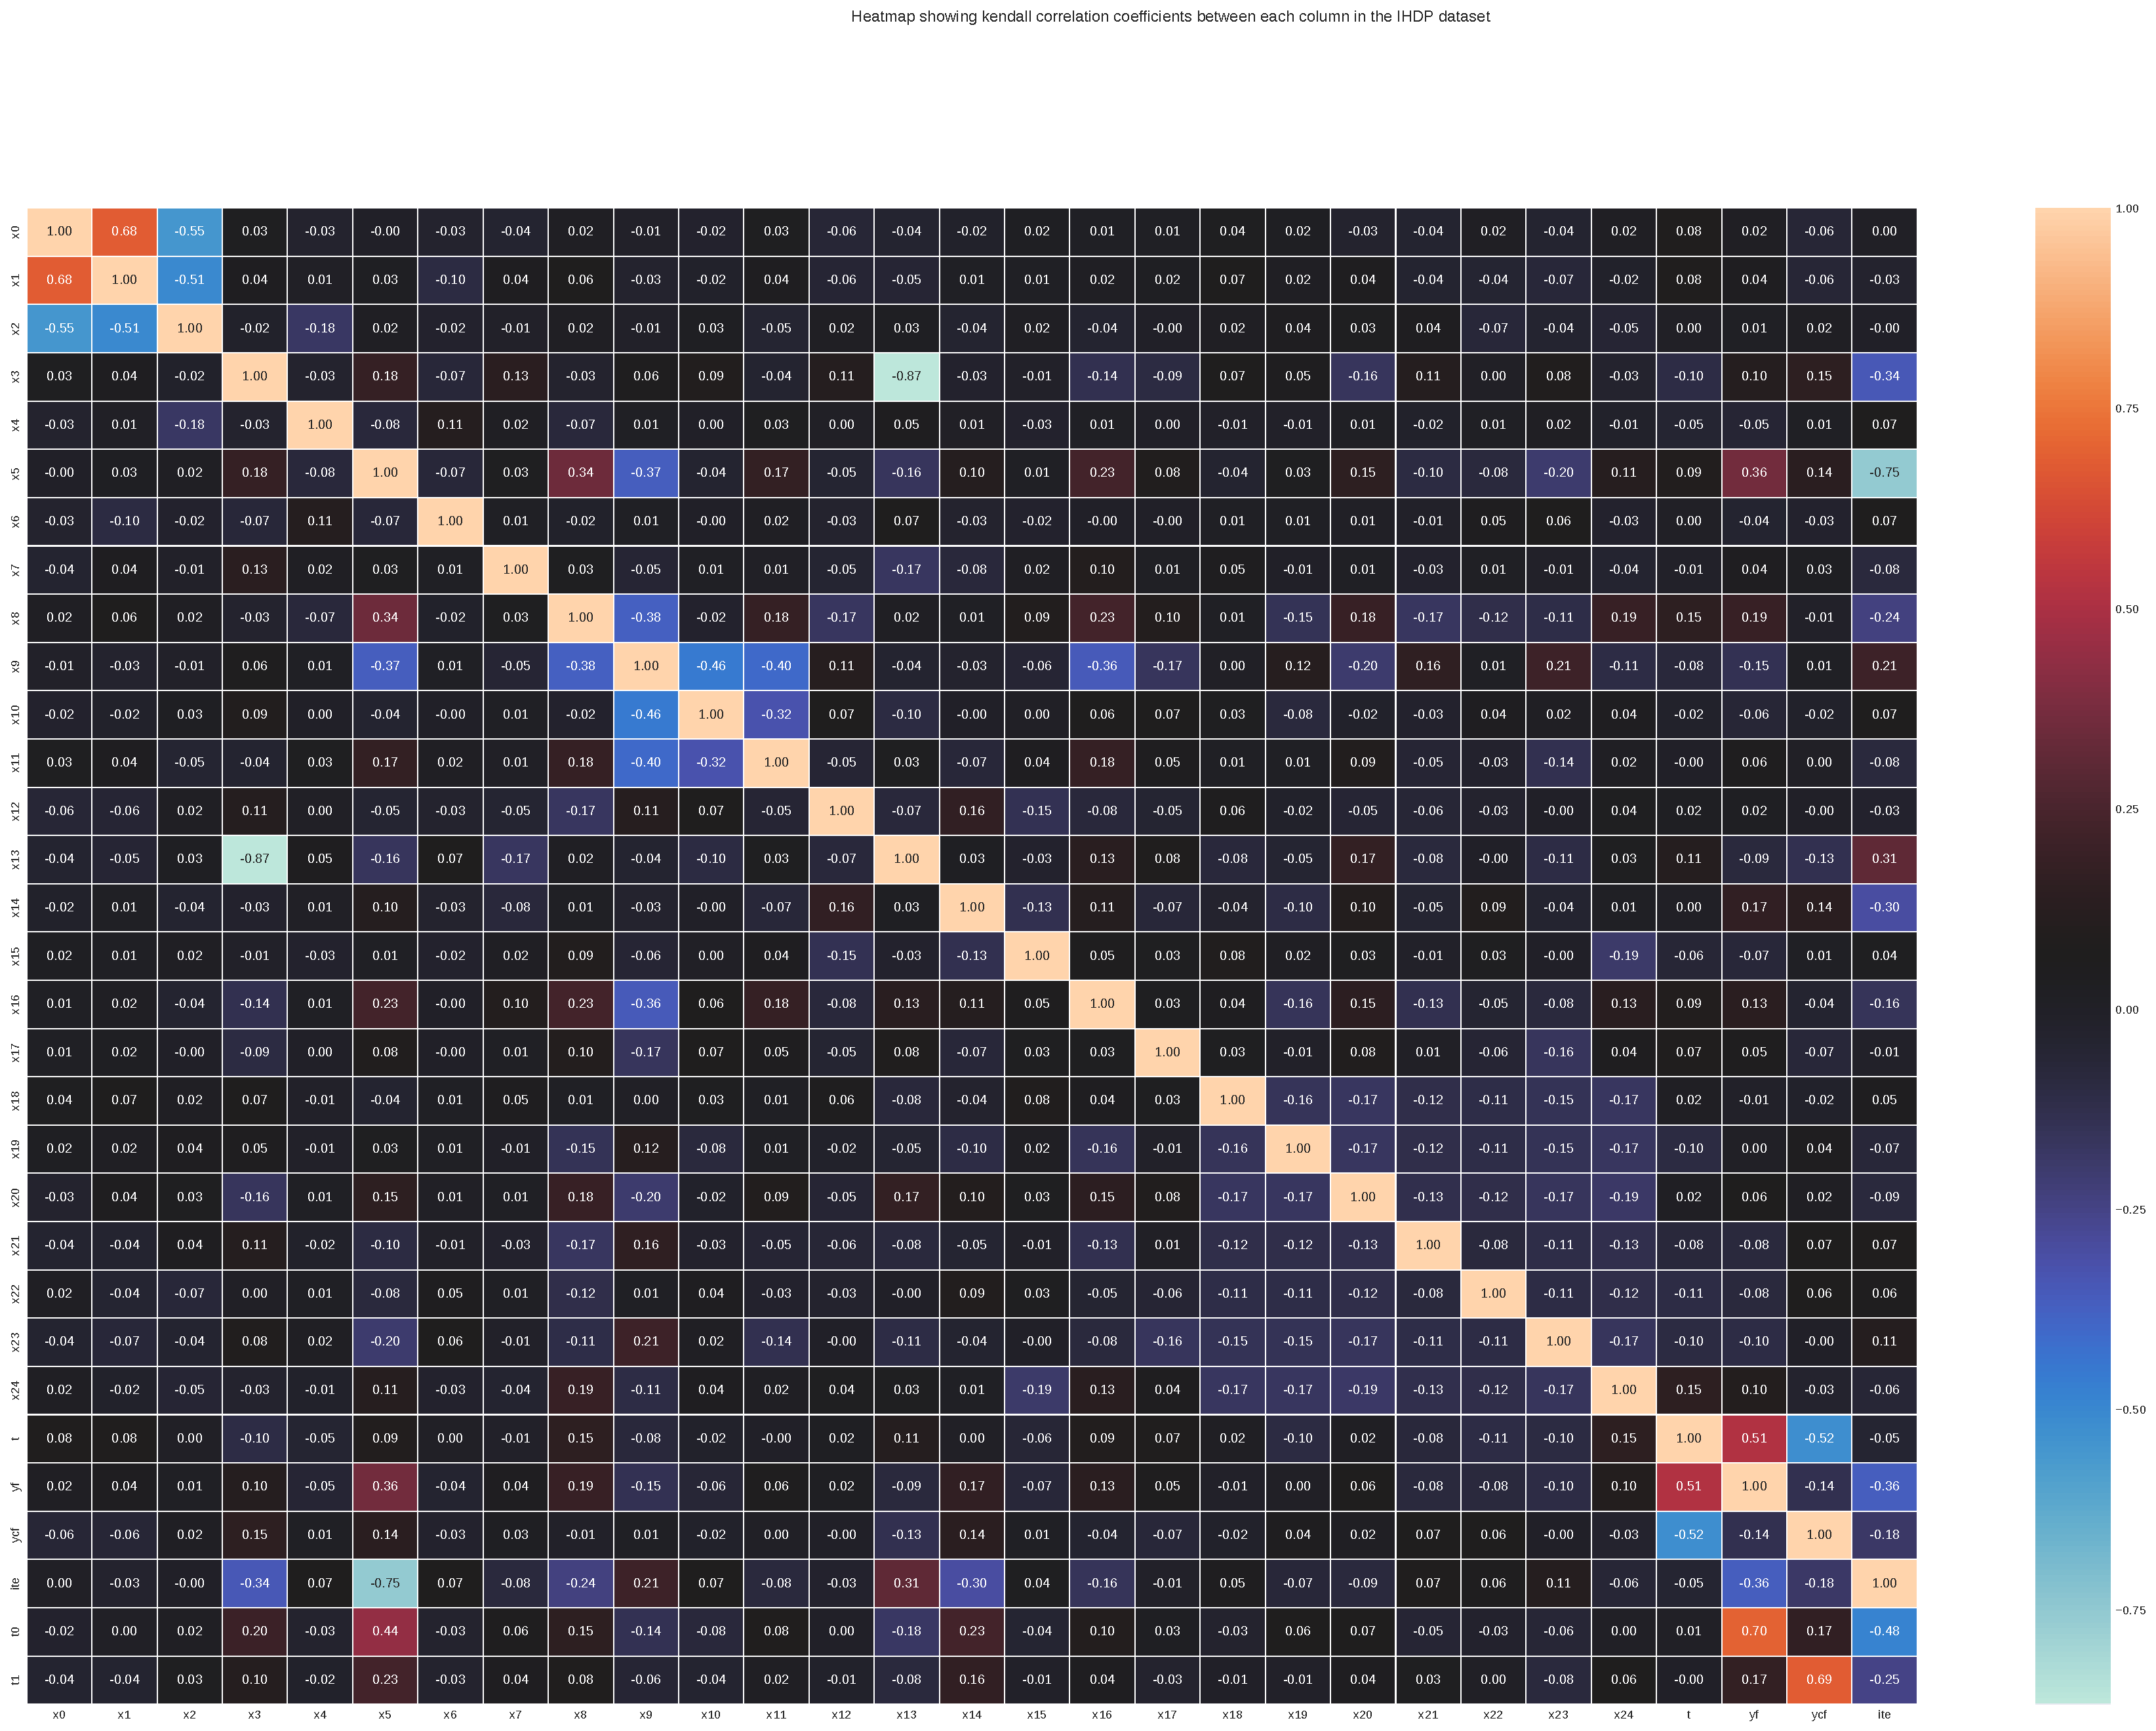
\includegraphics[width=1\textwidth]{project/data/ihdp_heatmap.pdf}
    \caption{
        \label{fig:ihdp_correlation}Correlation heatmap for the IHDP dataset
    }
    \small{
        This annotated heatmap shows the correlation coefficients for the values in each
        column of the IHDP dataset (along with additional \texttt{t0} and \texttt{t1} columns). 
        \texttt{t0} contains the \texttt{y} values for each individual for the case
        where \texttt{t=0}, and vice versa for \texttt{t1} (with these columns being included
        for ease of looking at overall treatment/control outcomes).
    }
\end{figure}

Looking at \ref{fig:ihdp_correlation}, we can see that there isn't much clear correlation
between the values of each column in the IHDP dataset, barring a few outliers.

There is a rather strong positive correlation between \texttt{t} and \texttt{yf} (with a
slightly stronger negative \texttt{t}/\texttt{ycf} correlation), indicating that
being in the treatment group correlates to a higher \texttt{y}, but whether or not this
is due to causation does need to be investigated further.

Another 'important' correlation needing investigating is the rather strong negative
correlation between \texttt{x5} and \texttt{ite} (and, in extension,
\texttt{x5}'s relation to \texttt{t0} and \texttt{t1}), to see if this correlation
truly indicates whether a higher \texttt{x5} can cause the treatment to have an
unintended effect. This correlation is also illustrated in \ref{fig:ihdpgraphs},
showing this strong downward trend. However, looking at the \texttt{x5}
data in \ref{fig:ihdpfact}, we can see some individuals with high \texttt{x5}
values in the untreated group achieved rather high \texttt{yf} scores (with a \texttt{x5}
and \texttt{yf} correlation of 0.5), so one could argue that the negative ITE correlation
could be due to the counterfactual simulation not allowing similar \texttt{ycf}
values to be reached.

Other notable correlations include a positive correlation between \texttt{x0} and \texttt{x1}
(the correlation between having the largest absolute magnitude in this dataset, of 0.85,
and both having a strong negative correlation to \texttt{x2}), and the rather strong negative
correlation between \texttt{x3} and \texttt{x13}. These correlations could be a sign of
causation between them, or they could be an indicator of an external confounder.

\subsubsection{The Causal Questions}

\begin{enumerate}
\item To what extent does each \texttt{x} predict \texttt{y}?
\item To what extent does \texttt{t} predict \texttt{y}?
\item To what extent do the \texttt{x} values predict each other?
\item To what extent do the \texttt{x} values predict the \texttt{ite} values?
\end{enumerate}

\subsubsection{Metrics to use}

As this dataset contains full counterfactual/ITE data, I am able to use Precision in
Estimation of Heterogenous Effect ($\epsilon PEHE$) and Average Treatment Effect ($\epsilon ATE$)
in order to measure the correctness of the learner's estimations of individual treatment
effects\cite{CE888_causal}.



\FloatBarrier



\subsection{JOBS}

\FloatBarrier

\begin{figure}[ht]
\centering
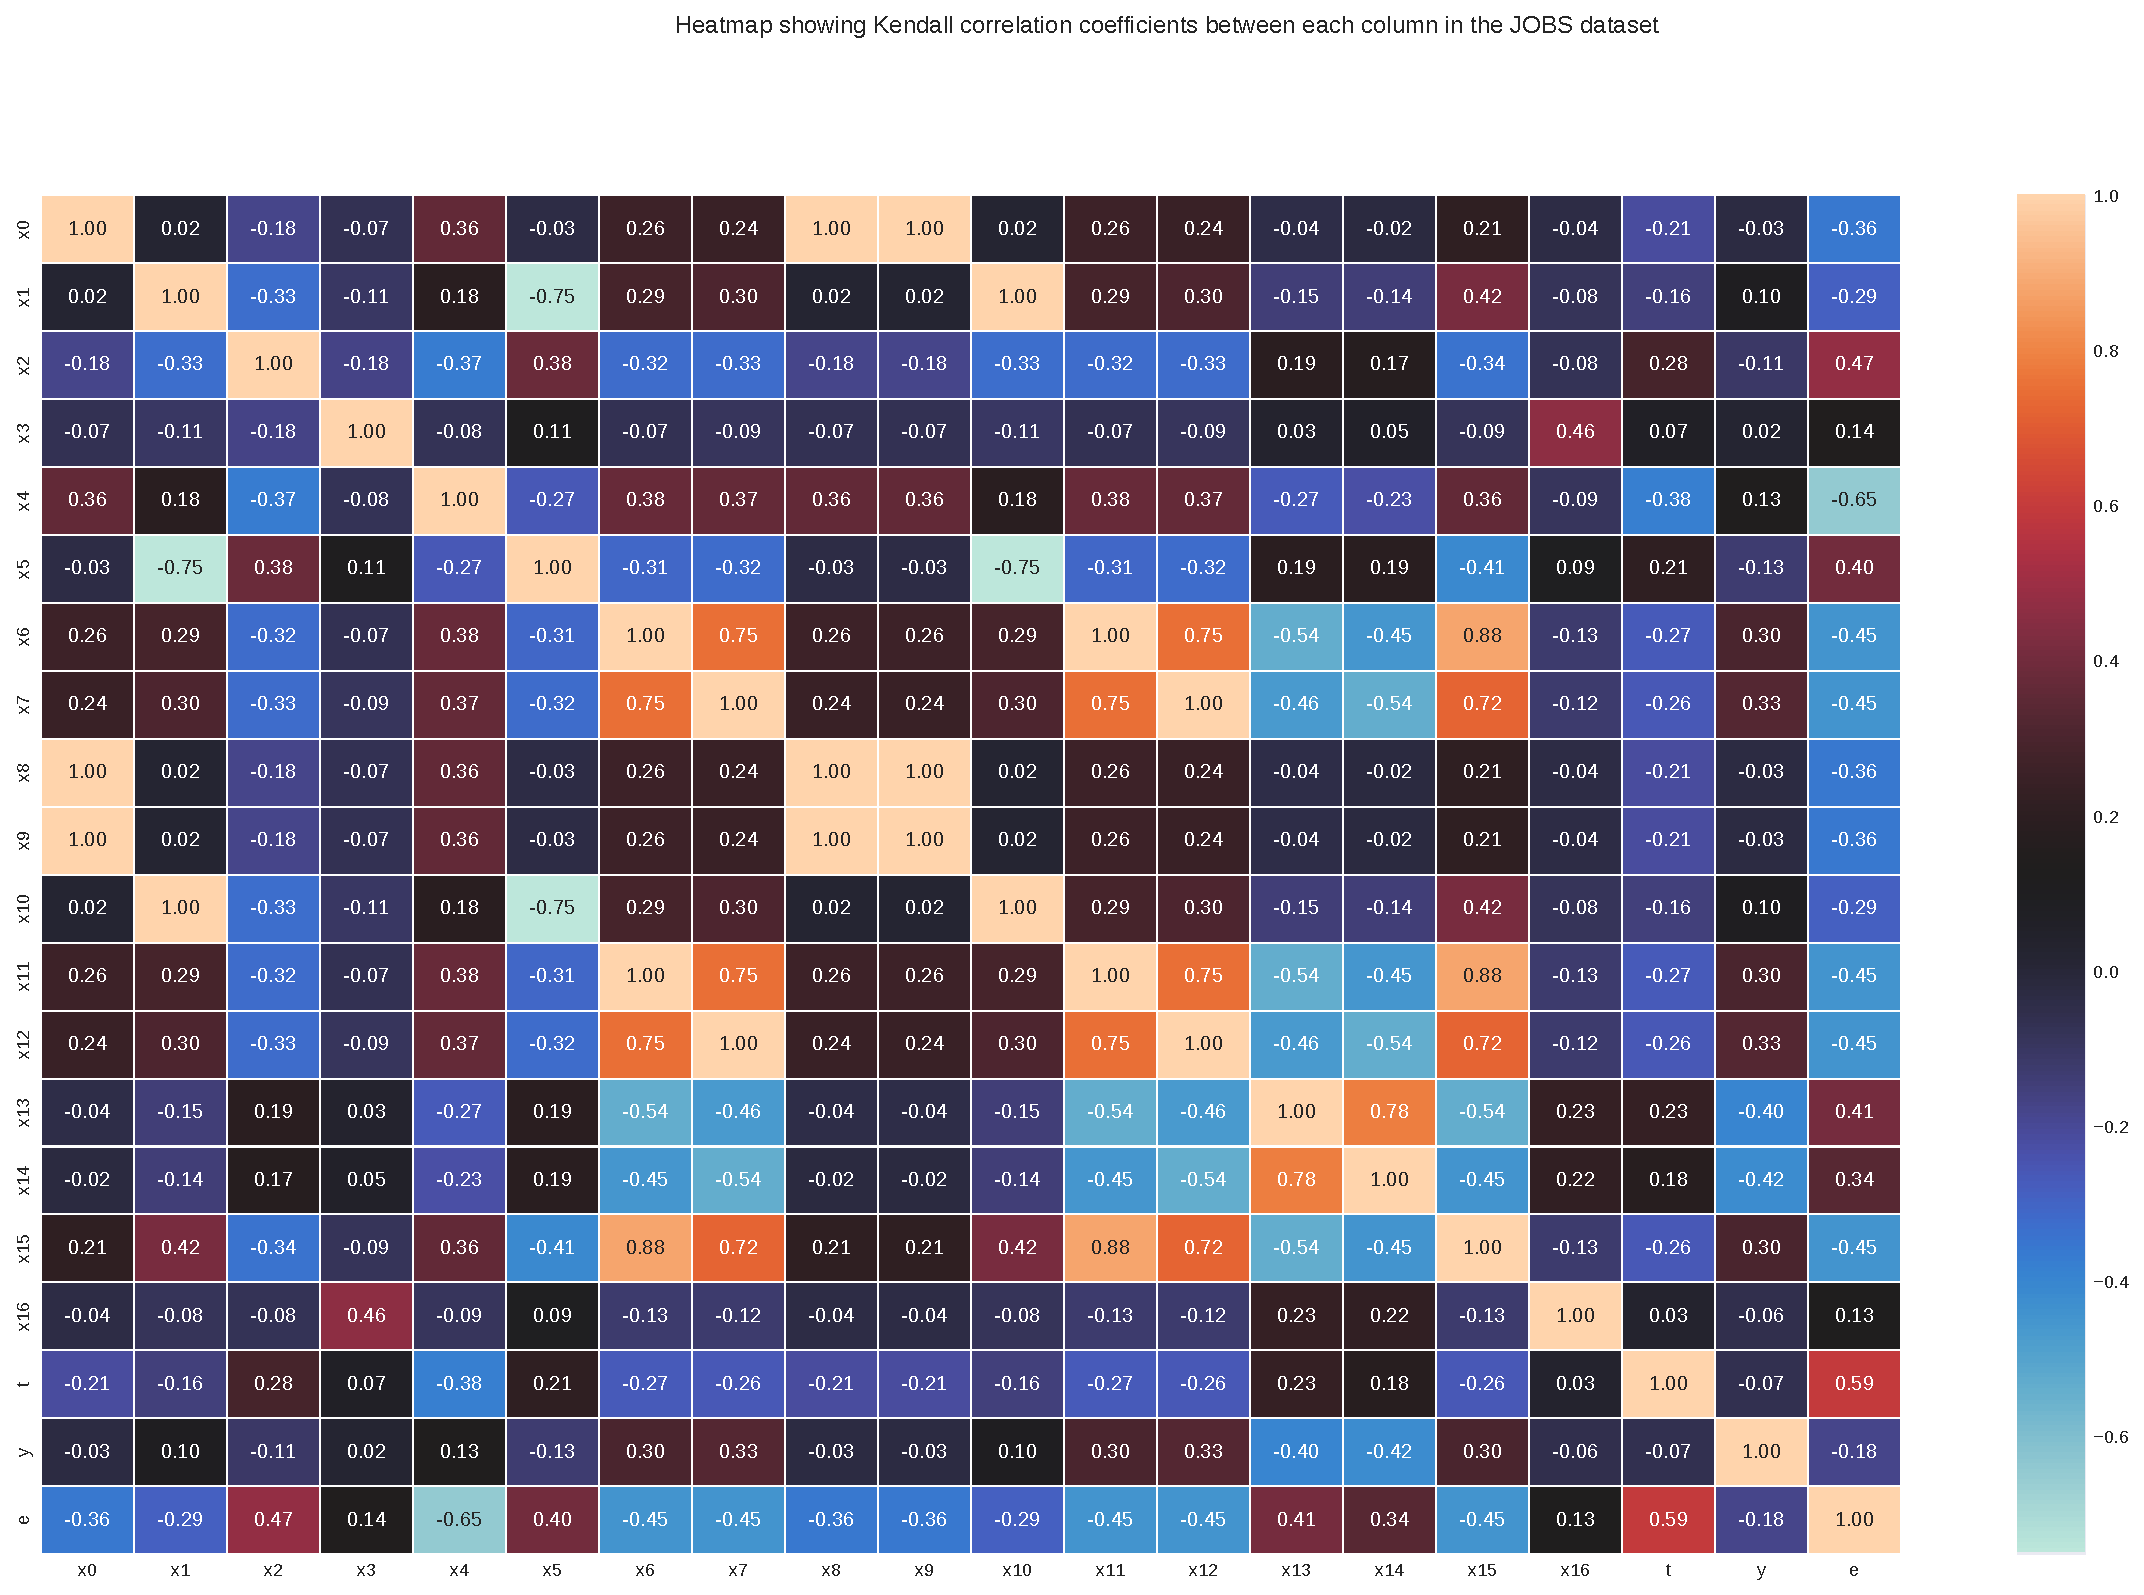
\includegraphics[width=1\textwidth]{project/data/jobs_heatmap.pdf}
\caption{\label{fig:jobs_correlation}Correlation heatmap for the JOBS dataset}
\end{figure}



\FloatBarrier

If you have only one dataset to work on, there is no need to add subsections to this section.
Otherwise, simply use the subsection command as shown in the tutorial below to create
separate subsections for each of the datasets.

The title of the subsection should be representative of the dataset (and not ``Dataset 1/2/3'').

Make sure you properly cite the origin of the dataset/s.

\section{Methodology}

\subsection{Preparing the learners}

\FloatBarrier

Before starting any training of the machine learners, I shall split the datasets into a learning
set (to use in training via K-fold cross validation) and a validation set.

Furthermore, for sake of consistency, I shall use an RNG instance with a seed of 42 for the
notebook, allowing reproducable results.

For the IHDP dataset, due to the rather small size of it, I shall use all of the counterfactual data as the validation set, along with ~10\% of the factual data (10\% of the treatment/control groups, aiming to stratify based on the ITE counterfactual data), leaving the remaining factual data available for k-fold cross validation training.

For the JOBS dataset, I shall use 20\% of the full data as the validation set (20\% of treatment/control, aiming to stratify based on the outcomes), leaving the remaining 80\% for training/testing.

When performing the testing, I shall be using scikit-learn's pipeline API, using pipelines with the structure explained in \ref{fig:pipeline}, for ease of re-running experiments, and allowing me
to take advantage of scikit-learn's \texttt{GridSearchCV} class, allowing me to experiment with
various hyper-parameter configurations whilst training the learners using k-fold cross validation.
In the interests of time, however, I may opt to use \texttt{HalvingGridSearchCV}, but the end
result of each process is identical.

\begin{figure}
    \centering
    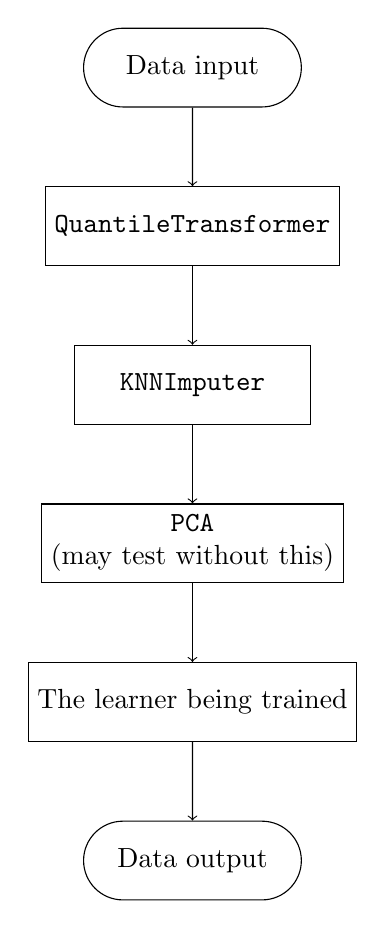
\begin{tikzpicture}
        \node[tRoundRect] (Start) {Data input};
        \node[tRect] (QTrans) [below =of Start] {\texttt{QuantileTransformer}} edge [<-] (Start);
        \node[tRect] (KNNImp) [below =of QTrans] {\texttt{KNNImputer}} edge [<-] (QTrans);
        \node[tRect] (PCA) [below =of KNNImp] {\texttt{PCA}\\(may test without this)} edge [<-] (KNNImp);
        \node[tRect] (Learner) [below =of PCA] {The learner being trained} edge [<-] (PCA);
        \node[tRoundRect] (Output) [below =of Learner] {Data output} edge [<-] (Learner);
    \end{tikzpicture}
    \caption{\label{fig:pipeline}Structure for the pipelines to be used for training}
\end{figure}

\FloatBarrier

\subsection{Simple Learners}

\quoteON

To obtain feature importances, I will attempt training a `RandomForestRegressor`,
an `ARDRegressor`, and a couple of `AdaBoostRegressor`s (consisting of the aforementioned
other regressors) to predict the `y` outcomes for individuals given their `x` attributes
and whether or not they have been treated (using `GridSearchCV` to handle hyper-parameter
optimization). The `RandomForestRegressor` shall be used due to how it conveniently provides a method for returning feature importances @\cite{sklearnensembleRandomForestRegressorscikitlearn102documentation}.
Obtaining these importances is slightly
more convoluted with the `ARDRegressor`, however, there is a workaround to obtaining these.
Despite the necessity of this workaround, the `ARDRegressor`, being a Relevance Vector Machine,
aims to perform regression by trying to weight the inputs based on evidence maximization,
in turn indirectly providing feature importances, without relying as much on a random seed.
\cite{Fletcher10relevancevector}\cite{sklearnlinearmodelARDRegressionscikitlearn102documentation}
The `AdaBoostRegressor` is an extension of these; effectively applying multiple instances of
the same regressor to the problem, weighting each one appropriately to catch the cases which
were missed by the previous regressors within the ensemble.
\cite{sklearnensembleAdaBoostRegressorscikitlearn102documentation}

The classification accuracy for this stage shall be assessed via `r2` scores,
comparing the predicted `y` for the individual (from their `x` and `t`) to the factual `y` value.
`r2` has been chosen due to how it provides a clear indicator of how good the estimator is compared
to returning the expected `y` value (on top of how close the estimator is to returning 'true' `y`
values), clearly indicating how good the predictions are.
\cite{sklearnmetricsr2scorescikitlearn102documentation}

Due to the `Jobs` dataset having `y` values of 0 and 1 only, I may instead approach it
as a classification problem rather than a regression problem. In this case, I would
use the 'Classifier' variants of the RandomForest and AdaBoost ensembles, but would
use a `LogisticRegression` learner instead of an `ARDRegressor` (as no classification
alternative to `ARDRegressor` exists)
\cite{sklearnlinearmodelLogisticRegressionscikitlearn102documentation}.
Furthermore, I would use the cross-entropy loss instead of r2 loss,
as cross-entropy still provides a clear indication of how close the classifier is to being
'perfect', and provides stronger penalties for inaccuracy as they get more inaccurate.
\cite{sklearnmetricsloglossscikitlearn102documentation}.

\subsection{Propensity Score re-weighting}

\quoteON

Similar to the 'Simple Learners' stage, I shall try using the identified classification models
to predict propensity scores for each dataset (by aiming to predict `t` given `x`), and then
using the identified 'best' classifier to predict what class they will be in (and giving that
to the Inverse Propensity Score function to produce the actual sample weights).
Unfortunately, due to the `ARDRegressor` not supporting sample weights, I will need
to replace it with a standard `BayesianRidge` regressor for this, but it has a similar end result
\cite{sklearnlinearmodelBayesianRidgescikitlearn102documentation}.

I will then repeat the process outlined in 'Simple Learners' with these weighted models,
and compare the results of the learners with weighted samples to the performance of the
unweighted learners. 

\subsection{Advanced CATE estimators}

\quoteON

I shall attempt to compare the performances of the 
`XLearner`\cite{econmlmetalearnersXLearnereconml0130documentation},
`CausalForestDML`\cite{econmldmlCausalForestDMLeconml0130documentation},
and `ForestDRLearner`\cite{econmldrForestDRLearnereconml0130documentation}
CATE models, implemented as part of EconML\cite{econml}.

\section{Conclusions}

Should not include subsections.

From here (included) to line 139, there is a tutorial for you to learn how to add tables,
figures, create subsections, etc.
You should delete all of that after reading it, and not submit it as part of your report.


\appendix
\section{Appendix: The visualizations of the datasets}\label{appendix:graphs}

These are located here, in the appendix, as the size of them is too big for \LaTeX to neatly
insert them within the main content of this report.

\subsection{IHDP dataset visualizations}


Here are the graphs for the IHDP dataset.

\FloatBarrier

\begin{figure}[H]
    \centering
    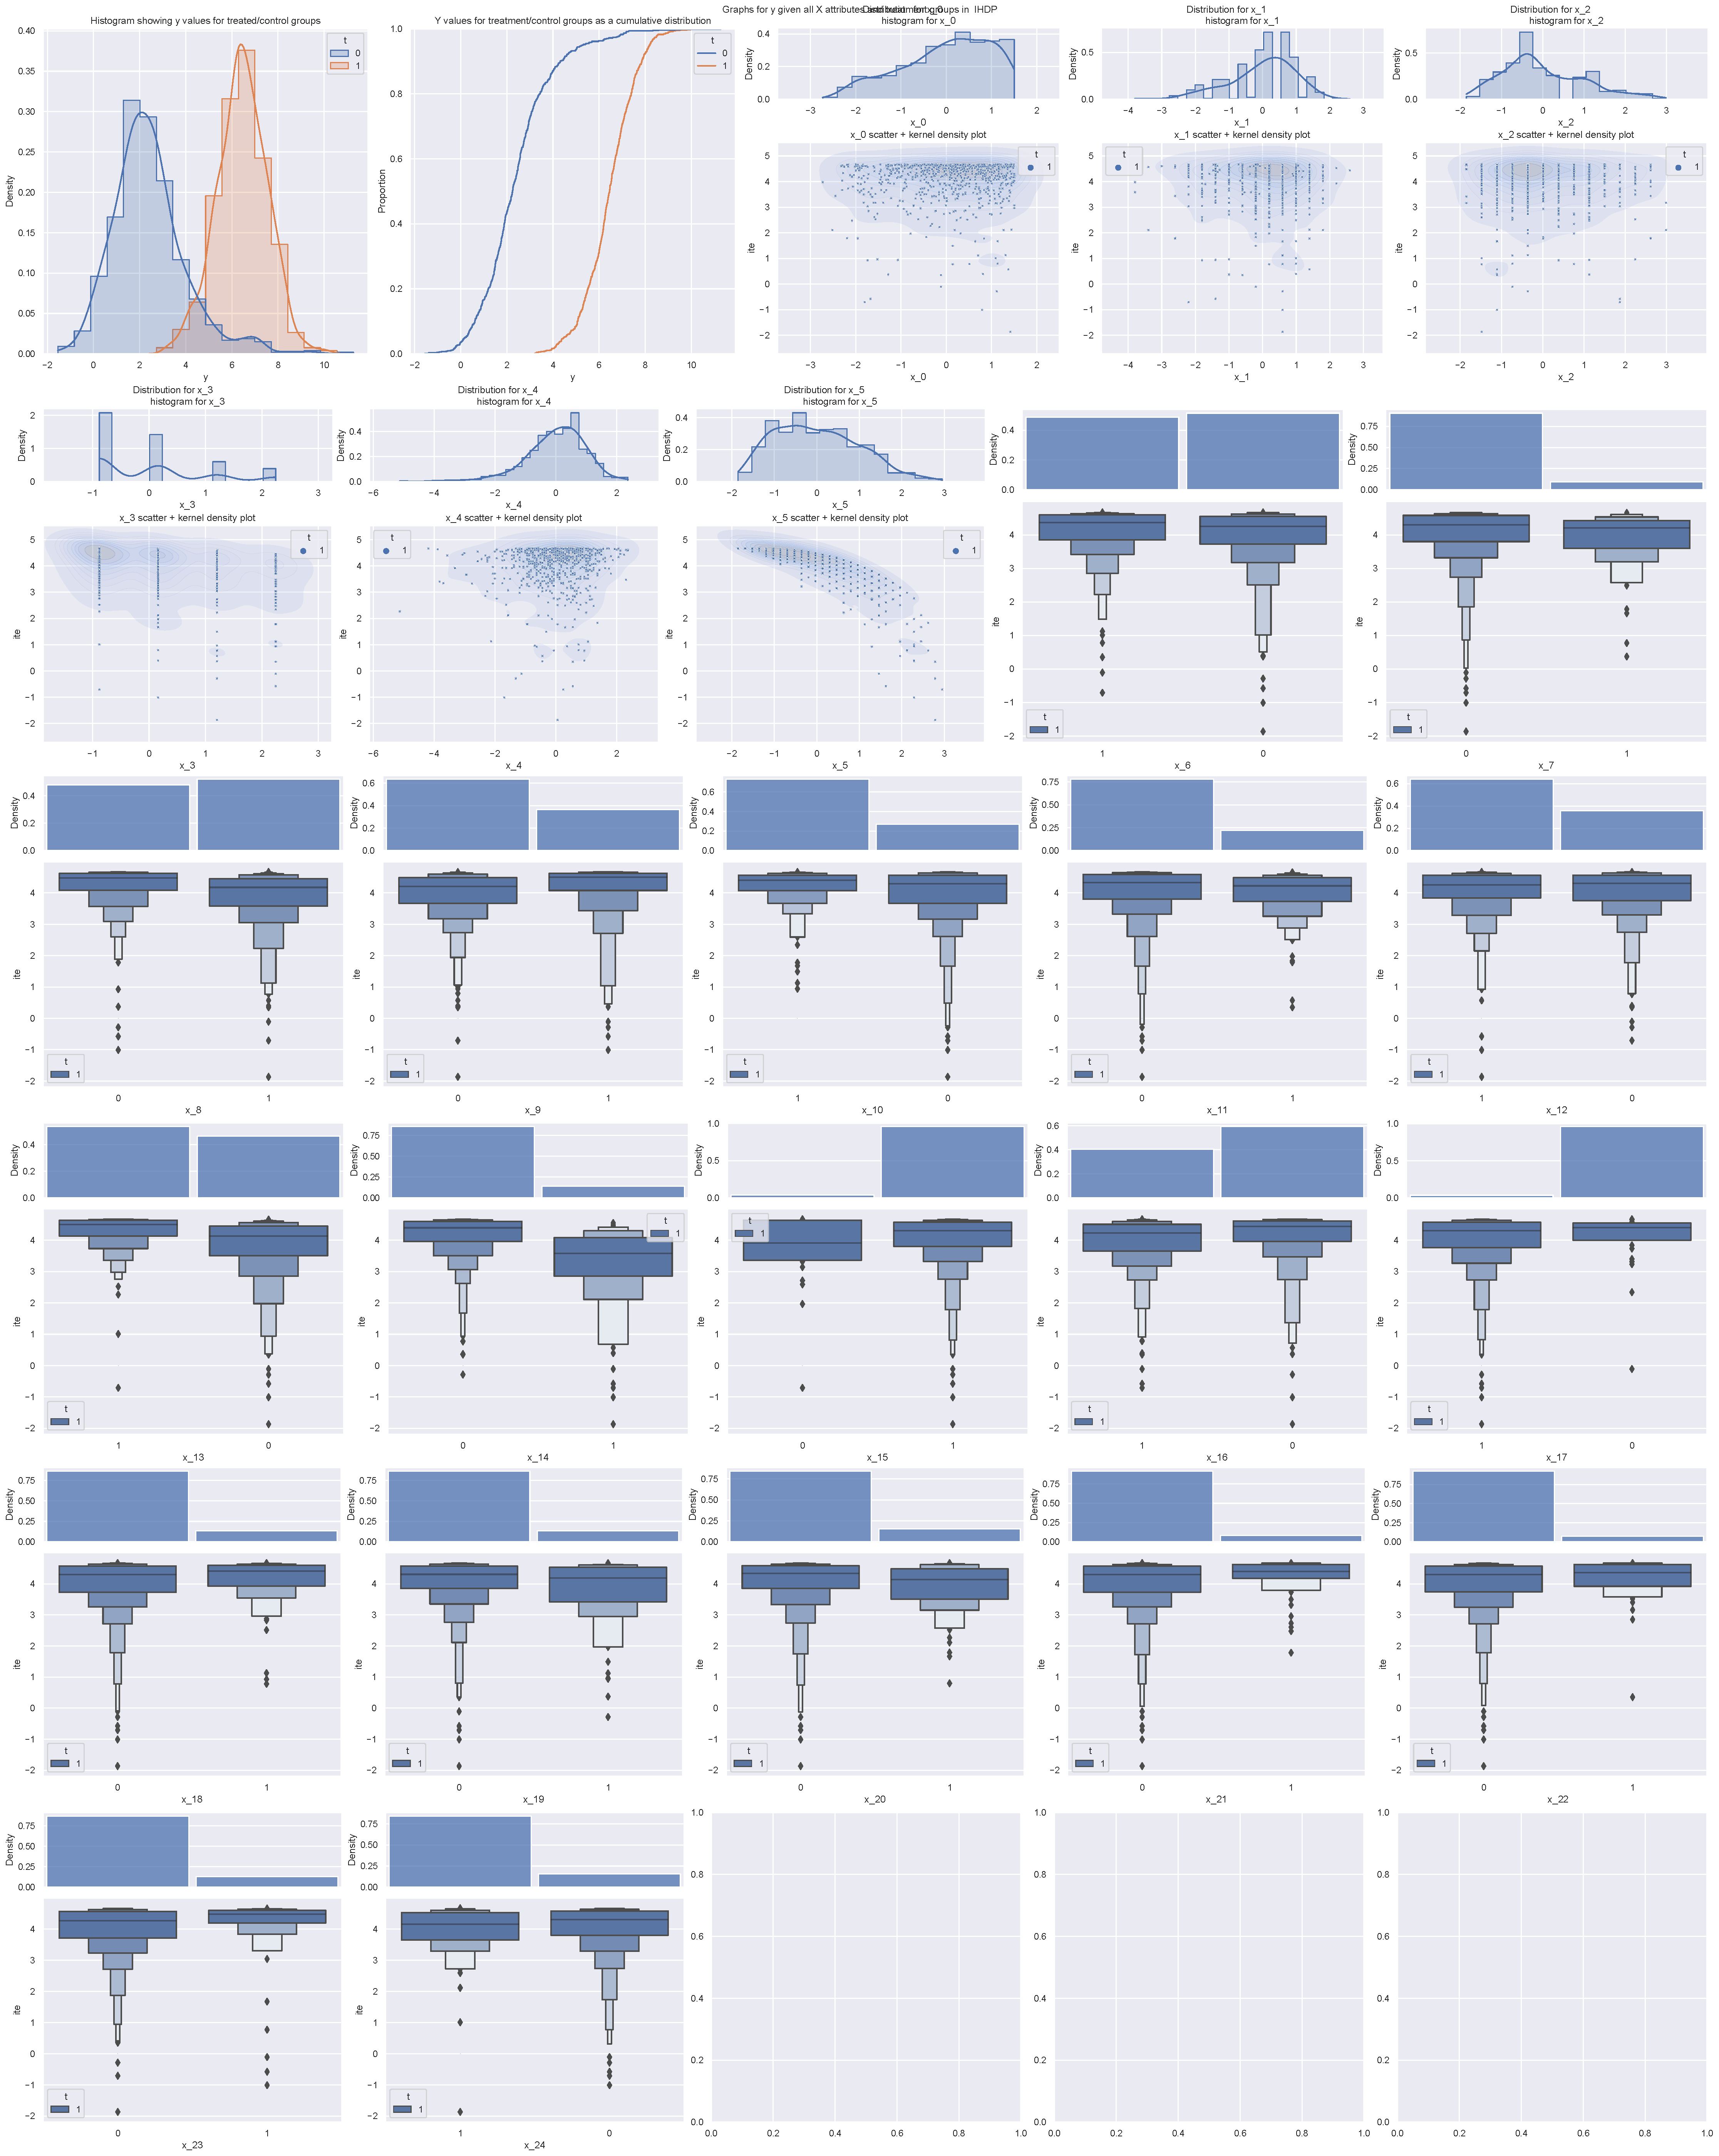
\includegraphics[width=1\textwidth]{project/data/ihdp_graphs.pdf}
    \caption{
        \label{fig:ihdpgraphs}Several graphs for the IHDP dataset, including counterfactuals
    }
\end{figure}

These graphs show how the \texttt{ite} values (along with \texttt{t0} and \texttt{t1})
vary for each individual, based on the value of each \texttt{x} variable for each individual. \texttt{t0}, \texttt{t1}, and \texttt{ite} are based on known counterfactual
data (end result being that \texttt{t0} contains the \texttt{y} value for the case where
the individual was in the control group, and vice versa for \texttt{t1}).

Looking at the density/regression plot between \texttt{t0} and \texttt{t1}, 
we can see a general improvement in the \texttt{y} scores for the population when
receiving the treatment, with few individuals falling below the \texttt{y=x diagonal}
line (these individuals being those who had a negative \texttt{ite}).

We can see a somewhat clear negative correlation between \texttt{x5} and \texttt{ite},
and we can also see that, for several of the binary-valued \texttt{x} values,
there is a rather large imbalance in the quantities of individuals in the dataset
who have each value, which could limit the amount of useful information we could
potentially gain from these variables.

\FloatBarrier

\begin{figure}[H]
    \centering
    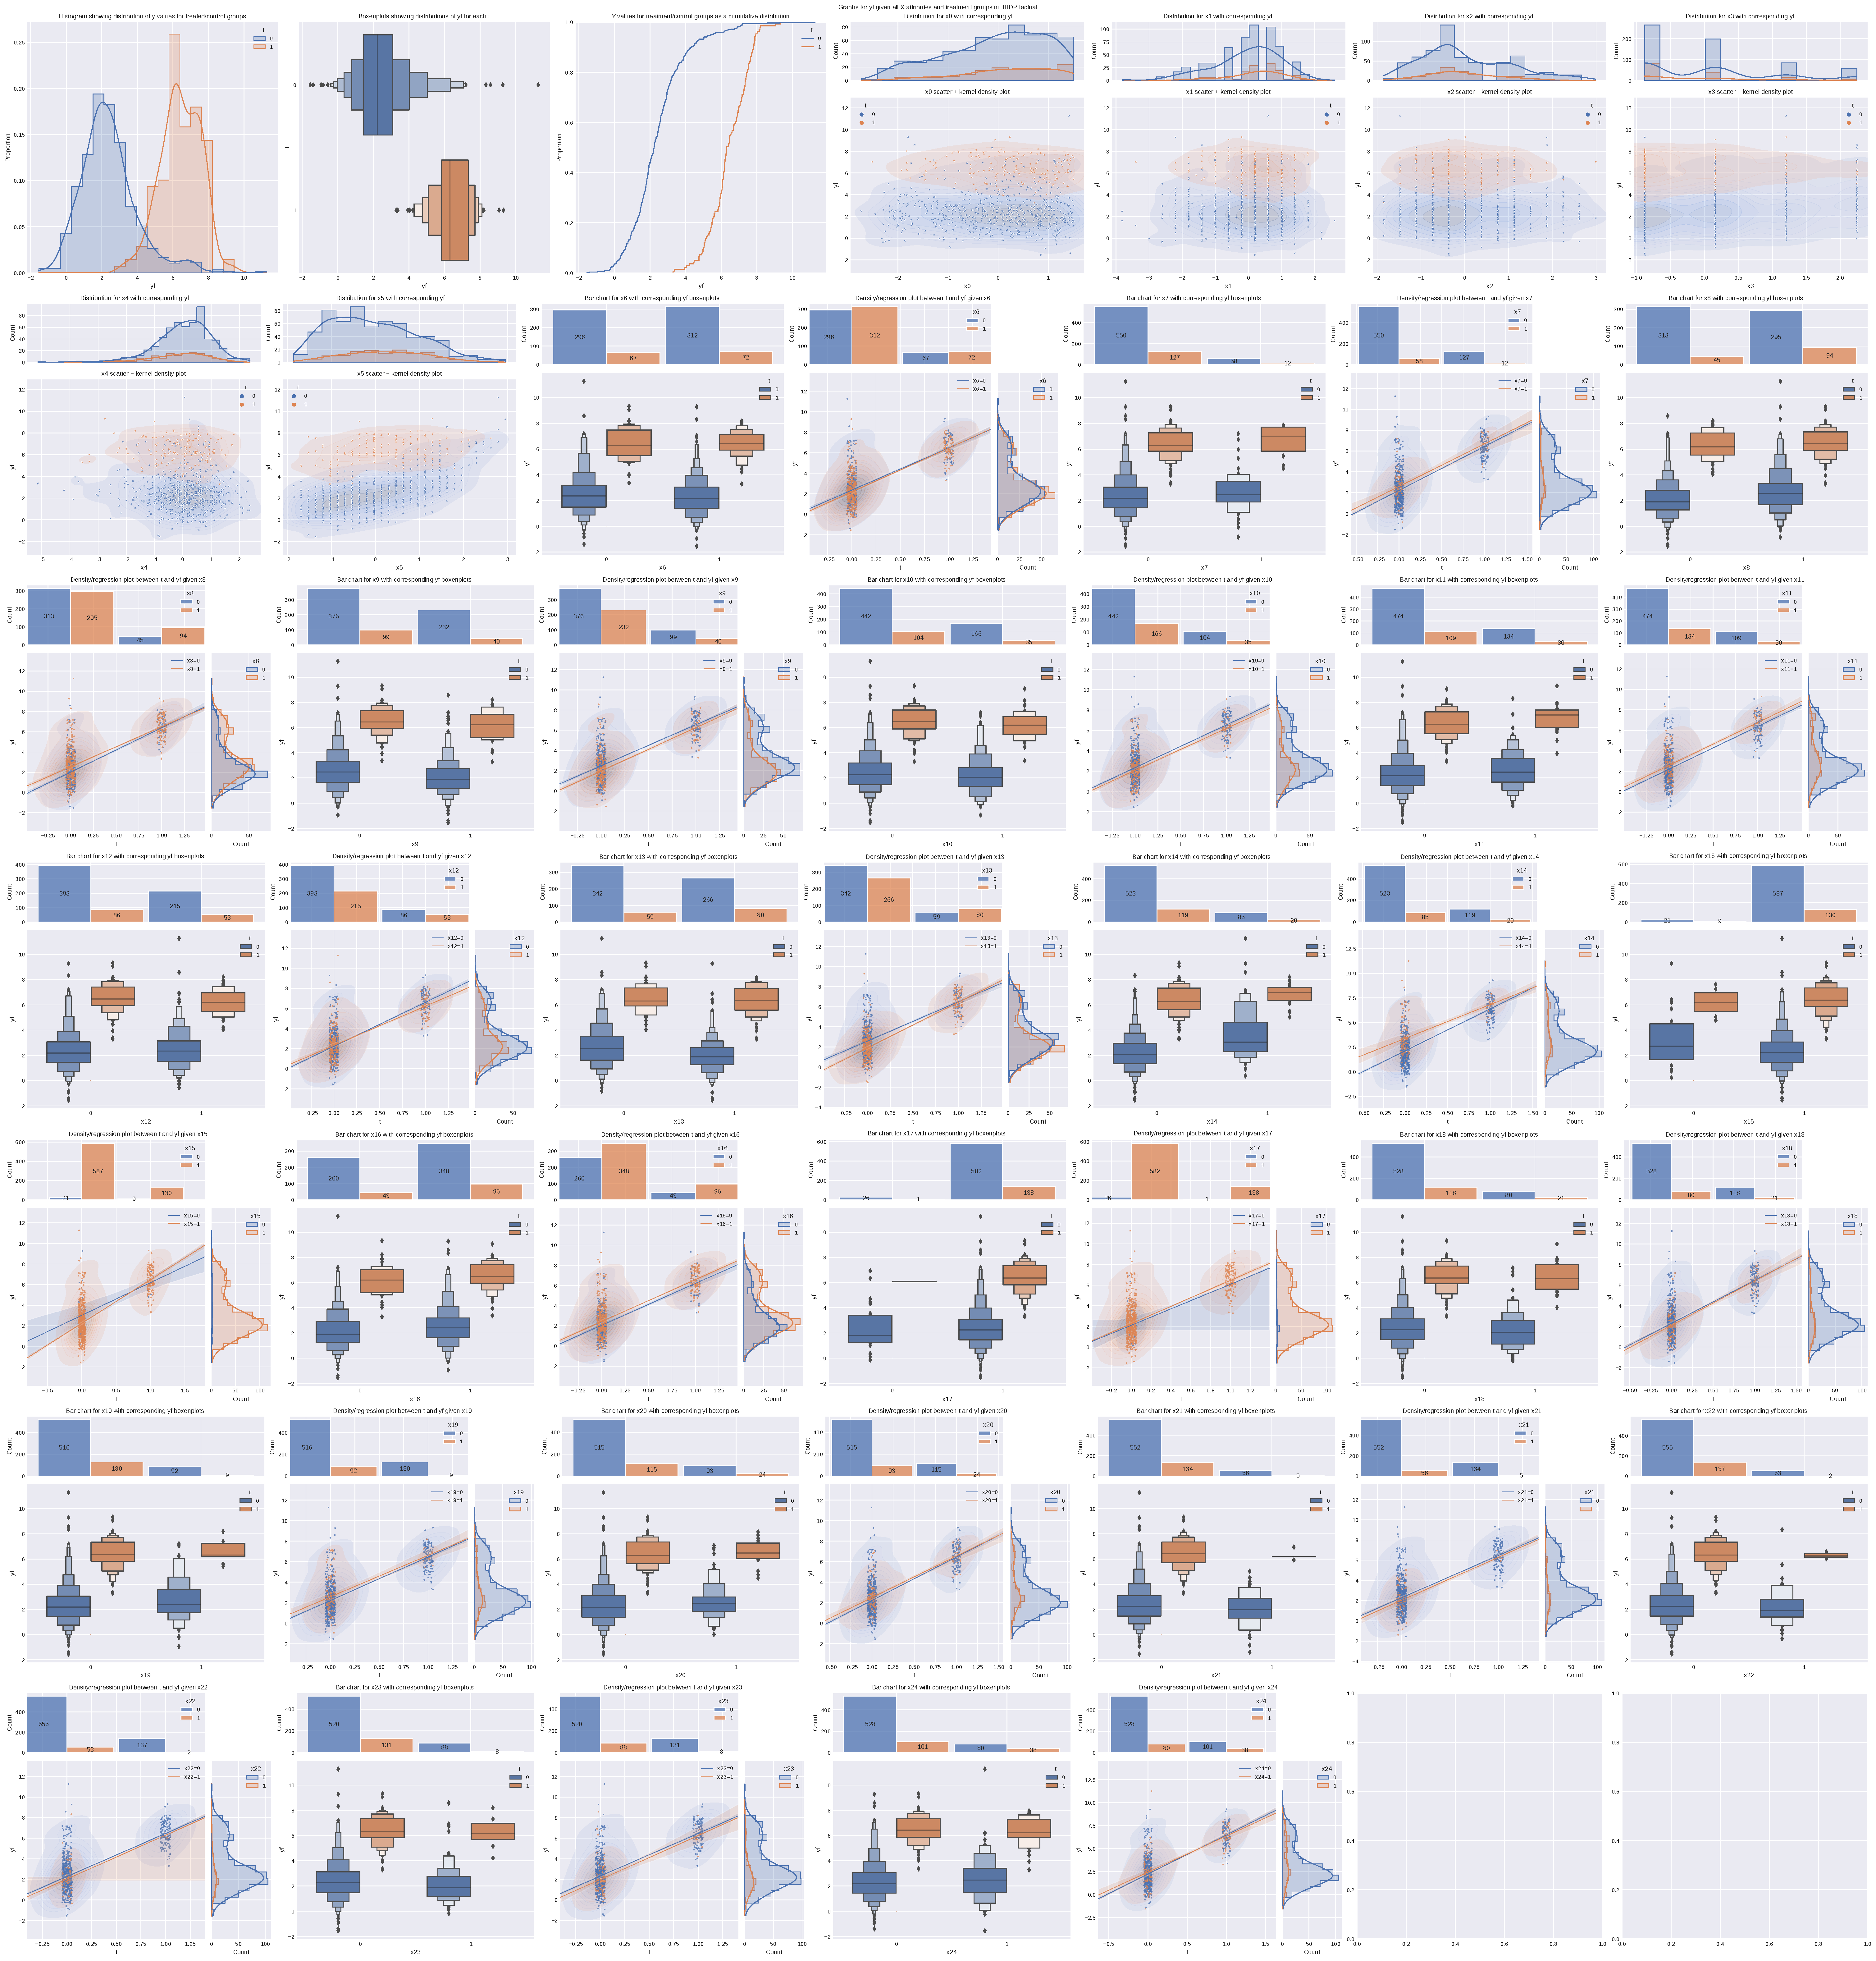
\includegraphics[width=1\textwidth]{project/data/ihdp_factuals.pdf}
    \caption{
        \label{fig:ihdpfact}Graphs for the factual data in IHDP
    }

\end{figure}

These graphs are of the factual data (\texttt{yf}) within the IHDP dataset.
These do illustrate the general positive correlation between individuals receiving
treatment and having a higher \texttt{yf} value, but also shows how imbalanced
this dataset is (most notably with \texttt{x17}, where only 27 individuals have
\texttt{x17==0}.
        
These graphs clearly illustrate that the treated individuals generally have higher
\texttt{yf} values than their untreated peers, with roughly similar interquartile
ranges for treatment/control groups with different values for each binary
\texttt{x} value (even in the extremely unbalanced cases).

\FloatBarrier

\begin{figure}[H]
    \centering
    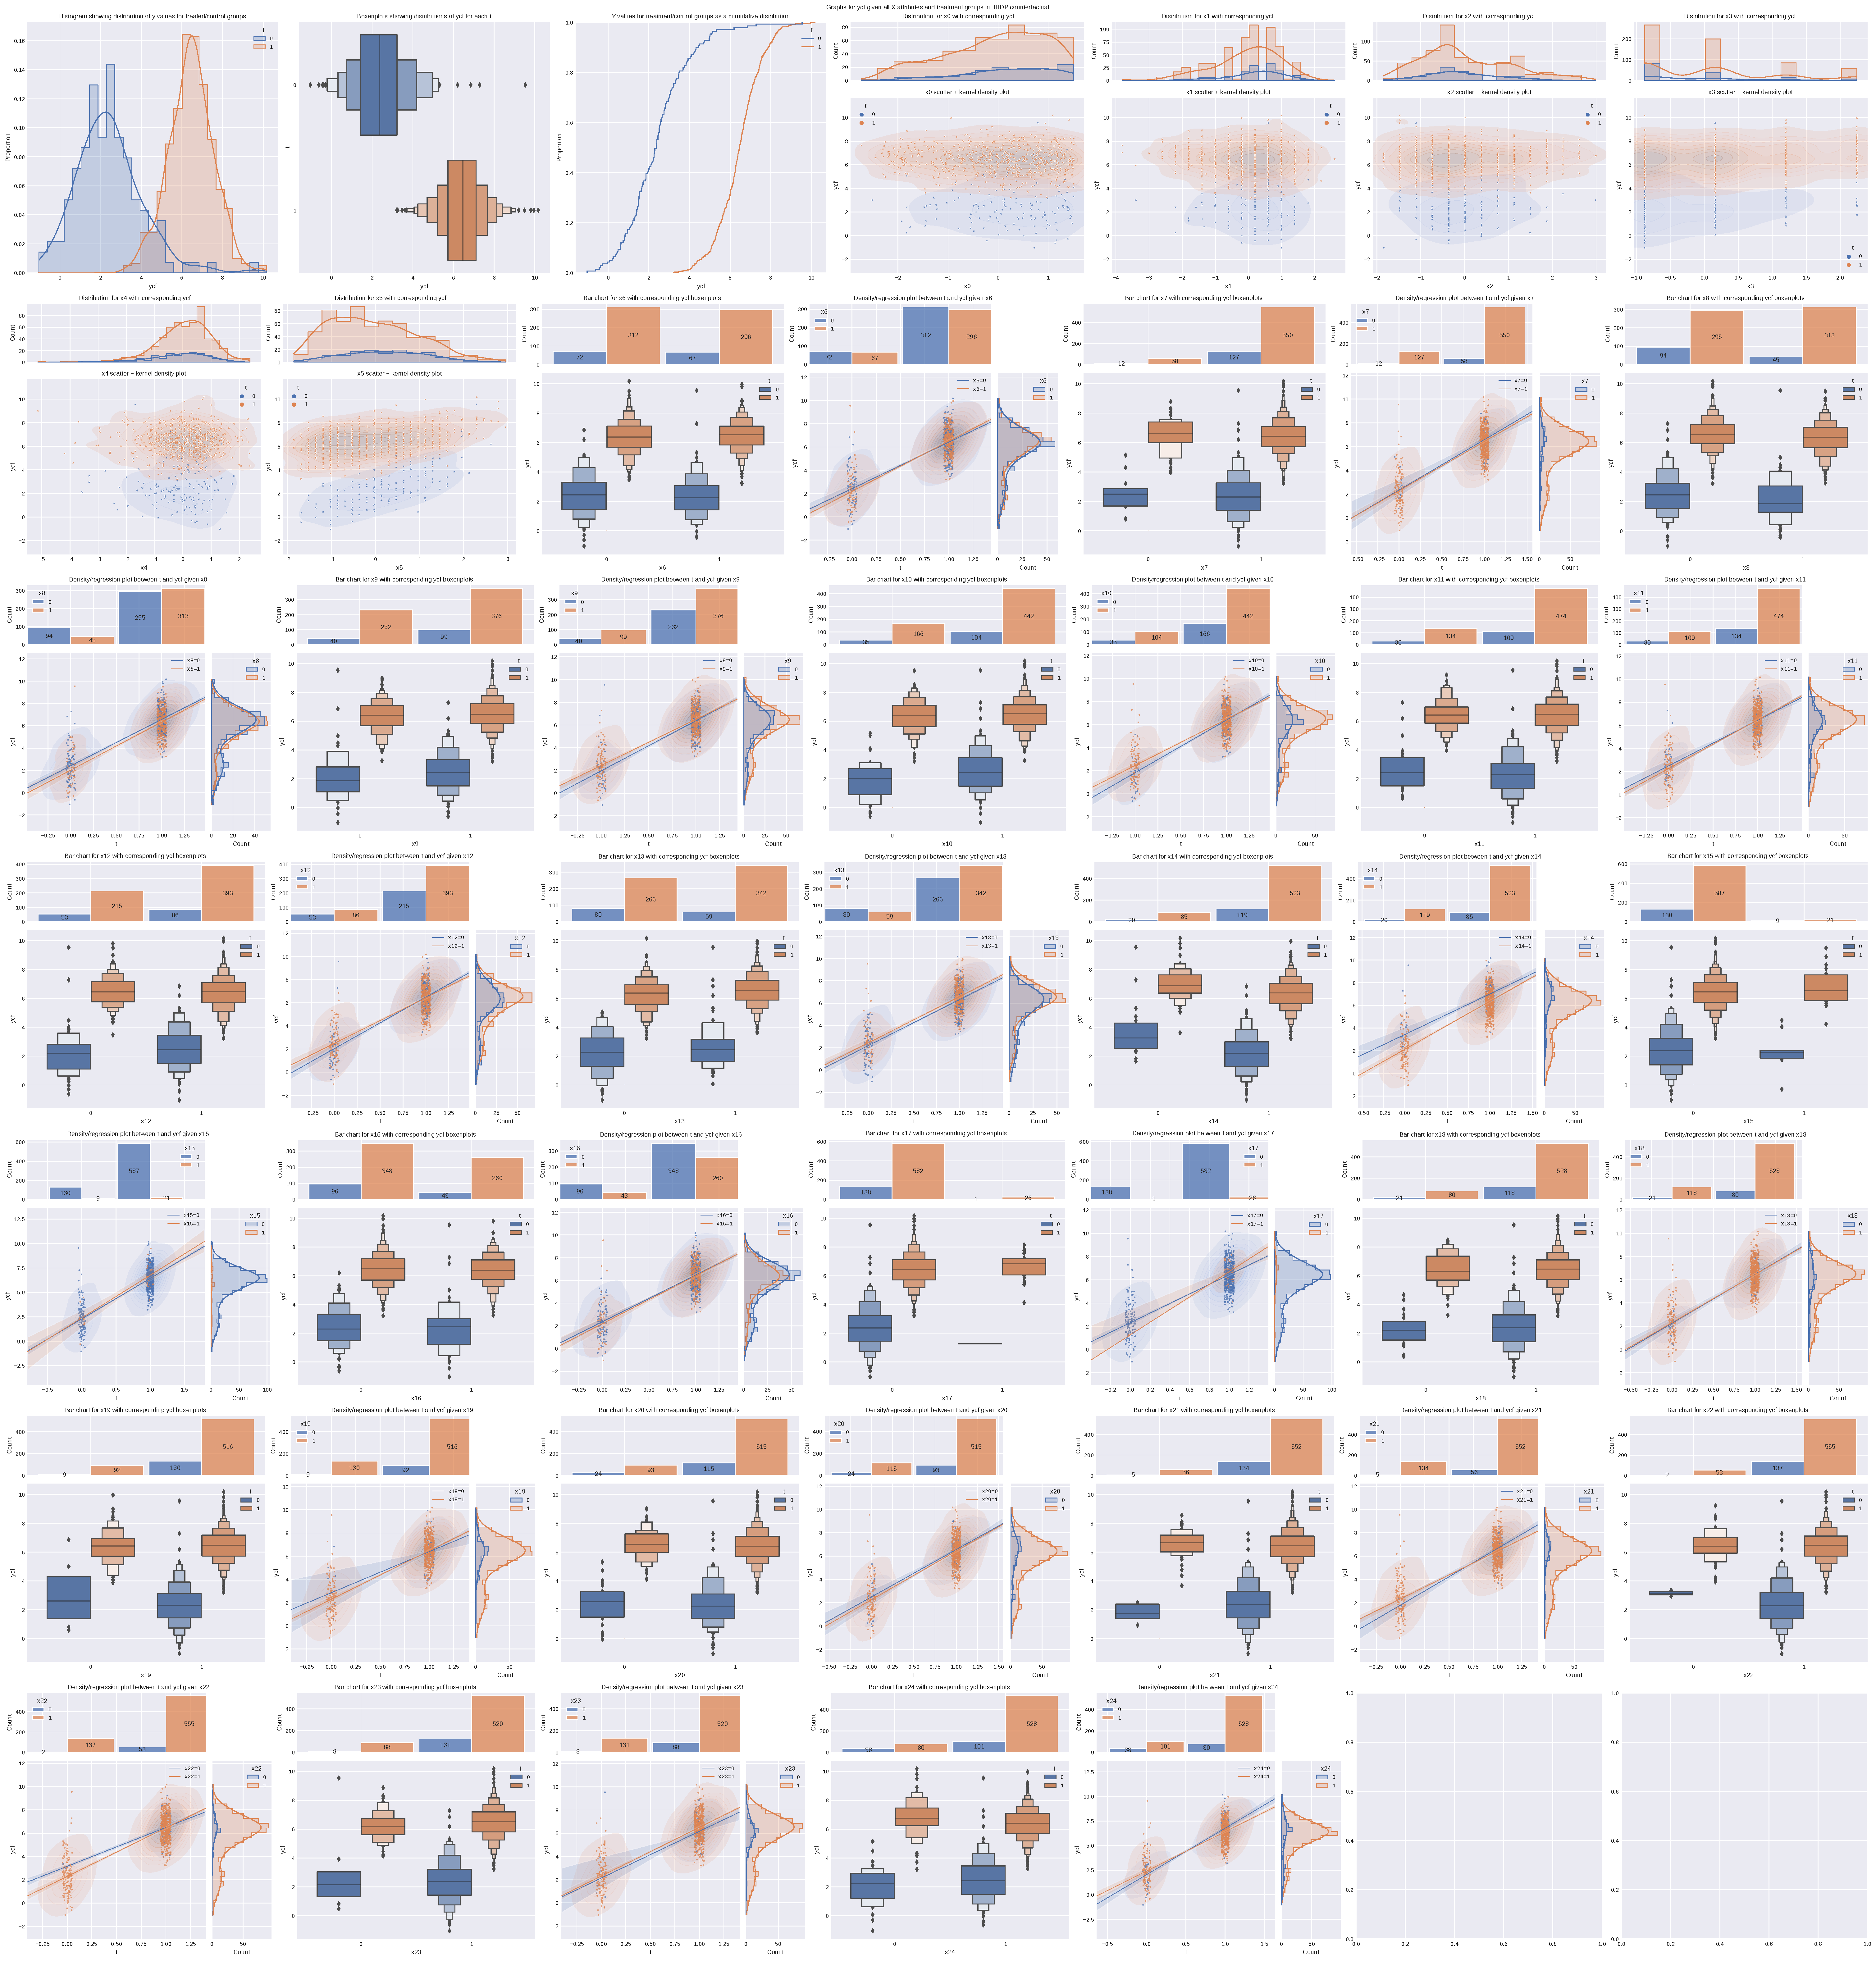
\includegraphics[width=1\textwidth]{project/data/ihdp_counterfactuals.pdf}
    \caption{\label{fig:ihdpcf}Graphs for the counterfactual data in IHDP}
\end{figure}

\FloatBarrier

\subsection{JOBS dataset visualizations}


Here are the graphs for the JOBS dataset.

\FloatBarrier

\begin{figure}[H]
\centering
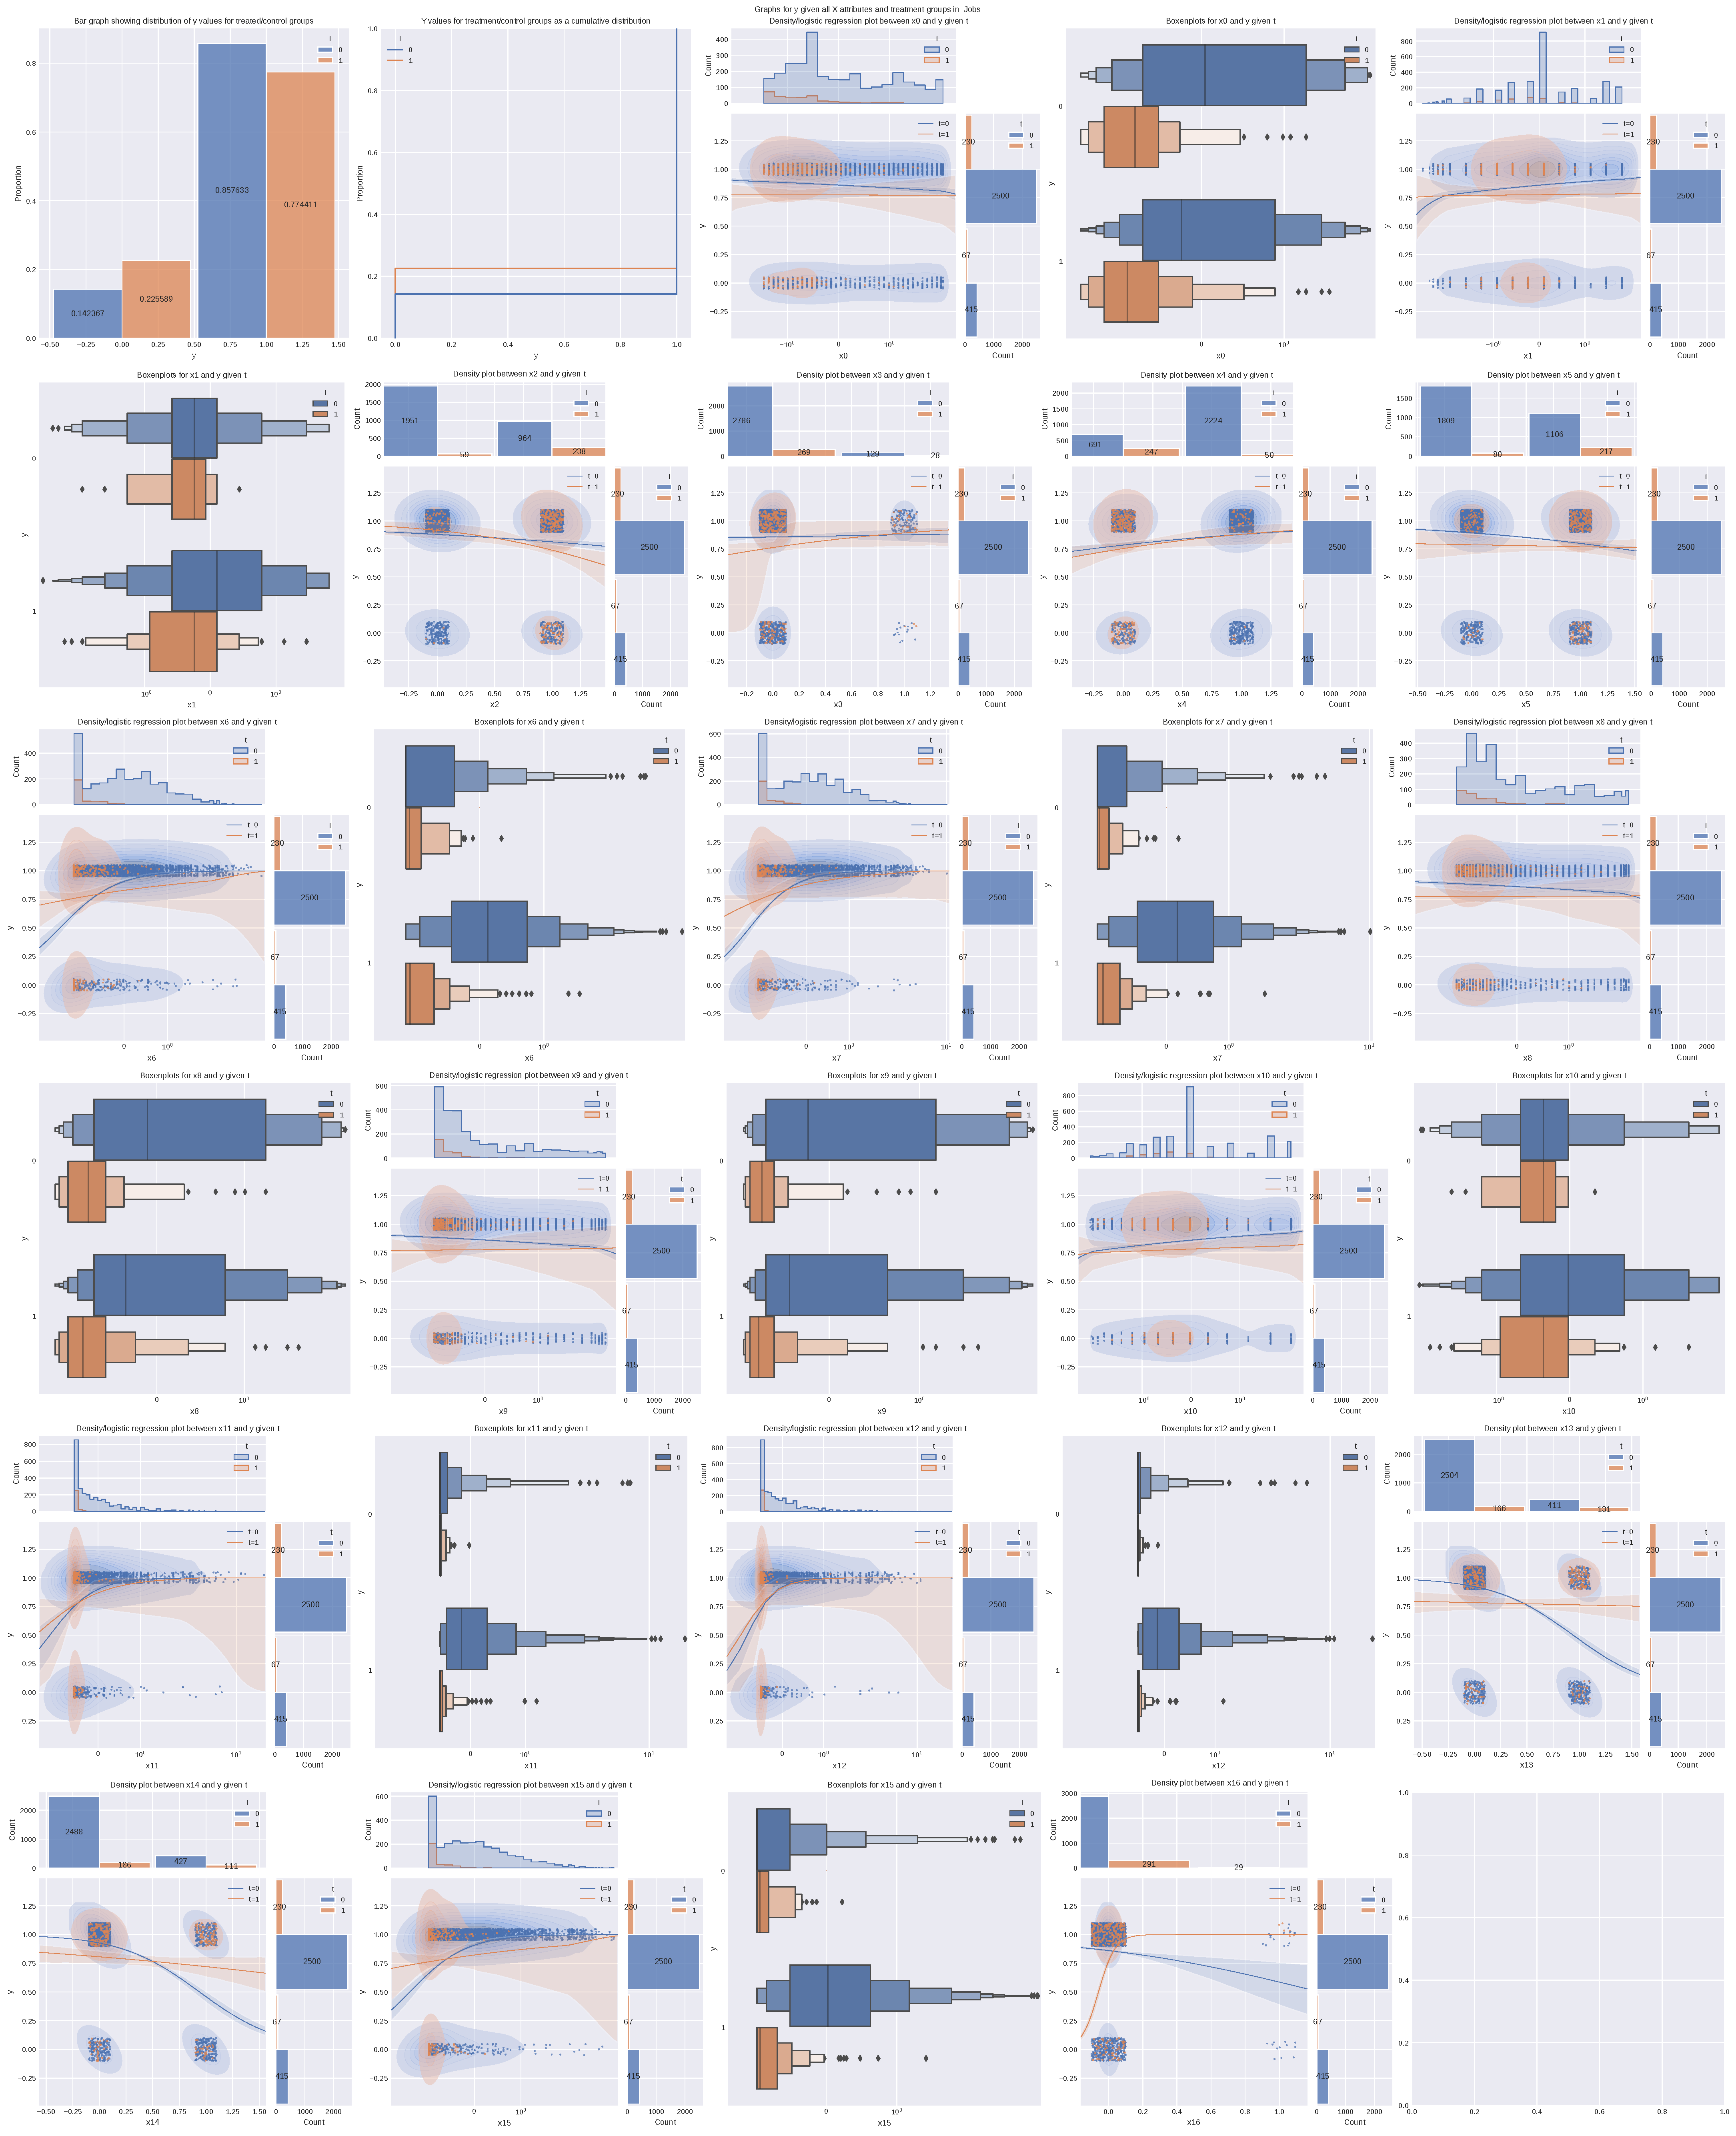
\includegraphics[width=1\textwidth]{project/data/jobs_graphs.pdf}
\caption{\label{fig:jobsgraphs}Several graphs for the JOBS dataset}
\end{figure}

\FloatBarrier


\section{Latex Tutorial}
\label{sec:tutorial}

To get the word count per section, you can use: \url{https://app.uio.no/ifi/texcount/online.php}

This section is only for you to learn how to write in LateX. Delete it after reading it.


\subsection{How to include Figures}

First you have to upload the image file from your computer using the upload link in the file-tree menu.
Then use the include graphics command to include it in your document.
Use the figure environment and the caption command to add a number and a caption to your figure.
See the code for Figure \ref{fig:frog} in this section for an example. Include the code for figures
and tables directly after the paragraph where you reference them.

\begin{figure}[tb]
\centering
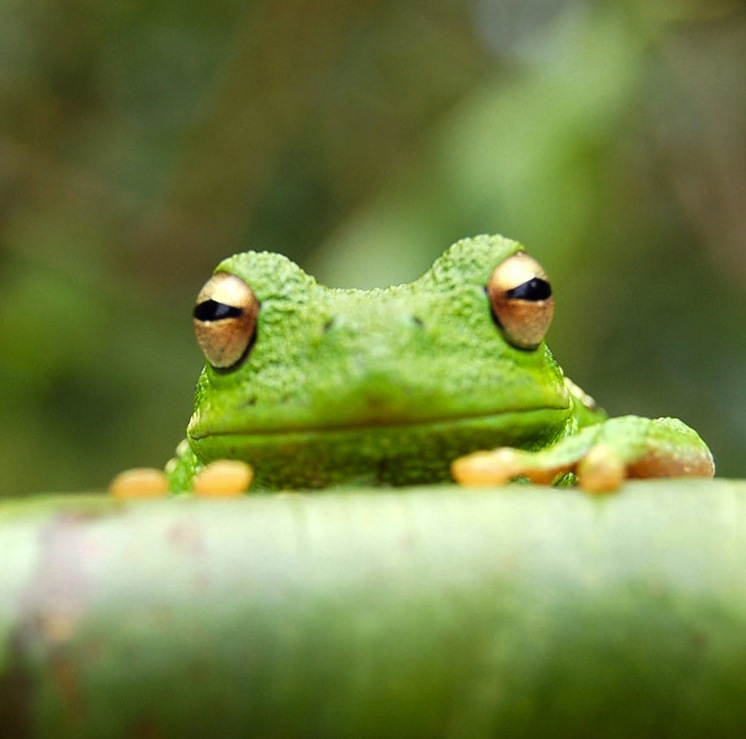
\includegraphics[width=0.3\textwidth]{frog.jpg}
\caption{\label{fig:frog}This frog was uploaded via the file-tree menu.}
\end{figure}

Note that your figure will automatically be placed in the most appropriate place for it,
given the surrounding text and taking into account other figures or tables that may be close by
(which is waaaay nicer than doing it on Word!).
You can find out more about adding images to your documents in this help article on
\href{https://www.overleaf.com/learn/how-to/Including_images_on_Overleaf}{including images on Overleaf}.



\subsection{How to add Tables}

Use the table and tabular environments for basic tables --- see Table~\ref{tab:widgets}.
For more information, please see this help article on \href{https://www.overleaf.com/learn/latex/tables}{tables}.

\begin{table}[tb]
\centering
\begin{tabular}{l|r}
Item & Quantity \\\hline
Widgets & 42 \\
Gadgets & 13
\end{tabular}
\caption{\label{tab:widgets}An example table.}
\end{table}


\subsection{How to add Lists}

You can make lists with automatic numbering \dots

\begin{enumerate}
\item Like this,
\item and like this.
\end{enumerate}
\dots or bullet points \dots
\begin{itemize}
\item Like this,
\item and like this.
\end{itemize}

\subsection{How to write Mathematics}

\LaTeX{} is great at typesetting mathematics. Let $X_1, X_2, \ldots, X_n$ be a sequence of independent and identically distributed random variables with $\text{E}[X_i] = \mu$ and $\text{Var}[X_i] = \sigma^2 < \infty$, and let
\[S_n = \frac{X_1 + X_2 + \cdots + X_n}{n}
      = \frac{1}{n}\sum_{i}^{n} X_i\]
denote their mean. Then as $n$ approaches infinity, the random variables $\sqrt{n}(S_n - \mu)$ converge in distribution to a normal $\mathcal{N}(0, \sigma^2)$.


\subsection{How to add Citations and a References List}

You can simply upload a \verb|.bib| file containing your BibTeX entries, created with a tool such as JabRef. You can then cite entries from it, like this: Just remember to specify a bibliography style, as well as the filename of the \verb|.bib|. You can find a \href{https://www.overleaf.com/help/97-how-to-include-a-bibliography-using-bibtex}{video tutorial here} to learn more about BibTeX.


\bibliographystyle{abbrv}
\bibliography{sample}

\end{document}